\documentclass[8pt]{beamer}

\usepackage{lmodern}
\usepackage[beamer,customcolors]{hf-tikz}

\tikzset{hl/.style={
    set fill color=red!80!black!40,
    set border color=red!80!black,
  },
}

\addtobeamertemplate{navigation symbols}{}{%
    \usebeamerfont{footline}%
    \usebeamercolor[fg]{footline}%
    \hspace{1em}%
    \insertframenumber/\inserttotalframenumber
}

\usetheme{Montpellier}
\usepackage[utf8]{inputenc}
\usepackage[english,american]{babel}
\usepackage{amsmath}
\usepackage{amsfonts}
\usepackage{amssymb}
\usepackage{graphicx}
\usepackage{booktabs}
\usepackage{float}
\usepackage{multirow}
\usepackage{subcaption}
\usepackage{threeparttable}
\usepackage{pdflscape}
\usepackage{lscape}
\usepackage{array} % for defining a new column type
\usepackage{tabulary}
\newcolumntype{K}[1]{>{\centering\arraybackslash}p{#1}}
	
%\author[Francisco Cavalcanti]{Francisco Cavalcanti\\\footnotesize{PUC-Rio}
%}

\author{
Flávia  Alfenas\\
\textit{PUC-Rio}\\ \vspace{3mm}
\and  
Francisco Cavalcanti\\
\textit{PUC-Rio}\\ \vspace{3mm}
\and   
Gustavo Gonzaga \\
\textit{PUC-Rio} 
}

\date{Junho, 2021}

\title{Dinamismo Econômico na Amazônia Legal \\ Uma análise entre 2012 - 2019}

\usepackage{tikz}
\def\checkmark{\tikz\fill[scale=0.4](0,.35) -- (.25,0) -- (1,.7) -- (.25,.15) -- cycle;} 

\newcommand{\quotes}[1]{``#1''}

\setbeamercovered{transparent} 
%\setbeamertemplate{navigation symbols}{} 
%\logo{} 
%\institute{} 
%\date{} 
%\subject{} 
\begin{document}

\newcolumntype{M}{>{\begin{varwidth}{4cm}}l<{\end{varwidth}}} %M is for Maximal column

\begin{frame}
\titlepage
\end{frame}

%\begin{frame}
%\tableofcontents
%\end{frame}

\section{Introdução}

\begin{frame}
\begin{itemize}
\item{Objetivo: aprofundar a discussão sobre o dinamismo econômico da Amazônia Legal a partir da identificação dos setores e ocupações que mais têm contribuído para a geração de emprego e renda na região}

\vspace{2mm}

\item{Caracterizar o dinamismo econômico da Amazônia Legal a partir das dimensões ocupacional e setorial disponíveis na base de dados da Pesquisa Nacional por Amostra de Domicílios Contínua (PNAD) do Instituto Brasileiro de Geografia e Estatística (IBGE)}
\end{itemize}
\end{frame}

\section{Metodologia}

\begin{frame}{}

\begin{itemize}
	\item{\textbf{Fonte dados}
			\begin{itemize}
			\item{{\footnotesize PNAD Contínua Trimestral (1T de 2012 até 4T de 2020)}}
			\end{itemize}					
		}	
		\vspace{2mm}
	\item{\textbf{Diferenças entre PNAD e PNAD Contínua}:		
		\begin{itemize}
			\item{{\footnotesize Mudanças metodológicas da PNAD e a Amazônia}}
			\item{{\footnotesize Processo de seleção da amostra}}
			\item{{\footnotesize Tamanho da amostra:}
				\begin{itemize}
				 	\item{{\scriptsize PNAD: 150 mil unidades domiciliares em um ano.}}
				 	\item{{\scriptsize PNAD Contínua: 200 mil unidades domiciliares em um trimestre.}}
				\end{itemize}
			}
		\end{itemize}					
		}
		\vspace{2mm}

	\item{\textbf{Amazônia Legal}
			\begin{itemize}
			\item{{\footnotesize RO, AC, AM, RR, PA, AP, TO, MT e MA (excluindo a região metropolitana e as regiões integrada de desenvolvimento econômico (RIDE)}}
			\end{itemize}					
		}
\end{itemize}

\end{frame}


\section{Importância relativa dos setores econômicos}

\begin{frame}[label=_importancia_relativa]

\begin{figure}
  \centering
  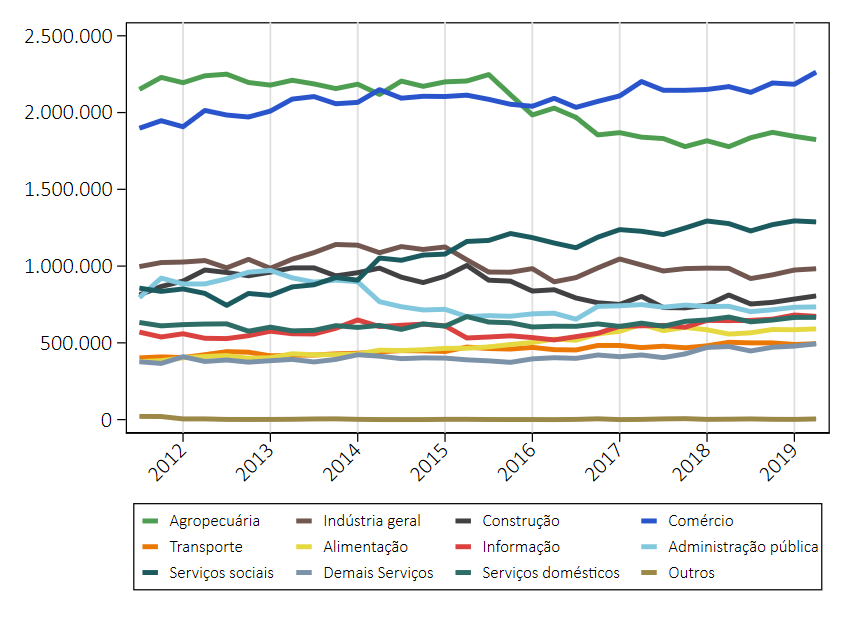
\includegraphics[width=.85\linewidth]{./../analysis/output/_importancia_relativa.png}
  \label{_importancia_relativa}
  \caption{{População ocupada por setor econômico, Amazônia Legal, 2012-2019}}
\end{figure}
\end{frame}



\begin{frame}[label=_importancia_relativa]

\begin{figure}
  \centering
  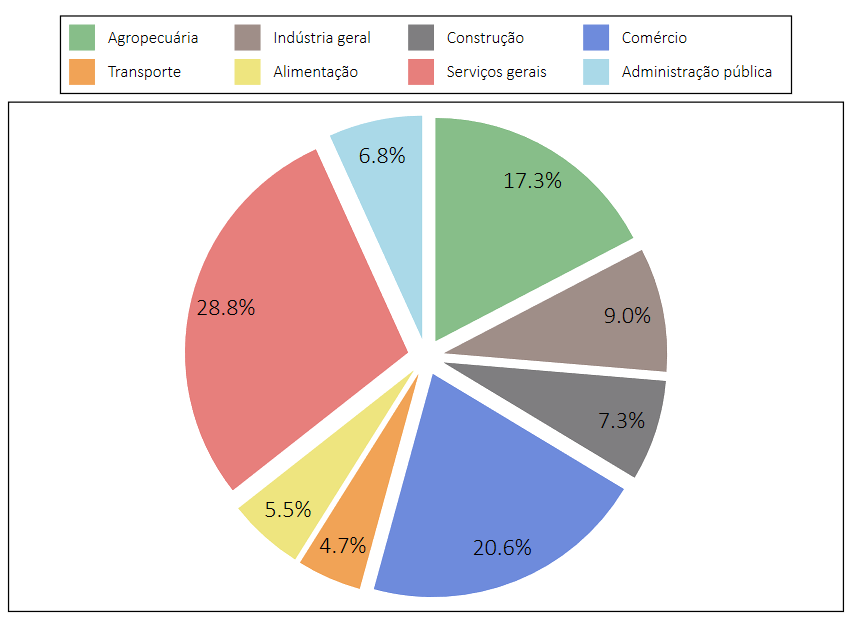
\includegraphics[width=.85\linewidth]{./../analysis/output/_importancia_relativa_pizza.png}
  \label{_importancia_relativa}
  \caption{{Proporção da população ocupada por setor econômico, Amazônia Legal, 2019}}
\end{figure}
\end{frame}


\begin{frame}[label=amzcod2dig]{}

\begin{table}[H]
\centering
\label{amzcod2dig}
\scalebox{0.85}{
\begin{threeparttable}
\caption{Variação e contingente da população ocupada, Amazônia Legal, 2012-2019}
\begin{tabular}{l*{8}{r}}
\midrule \midrule
 &  \multicolumn{3}{c}{\textbf{Variação 2012-19}} & \multicolumn{4}{c}{\textbf{2019}} \\
\cmidrule(lr){2-4} \cmidrule(lr){5-8}
 & Emp. & Emp. & Rendi. & { Emp.} & { Rendi. } & {Formal} & {Privado} \\
                    &       total&        (\%)&        (\%)&    {total }&     {(R\$)}&        (\%)&        (\%)\\
\hline
\\
\textbf{Amazônia Legal}               &     537.822&         5,3&         3,4&  10.632.195&       1.692&        40,6&        84,2\\
\\
\bottomrule
\end{tabular}
\begin{tablenotes}
\item \scriptsize{Fonte: com base nos dados da PNAD Contínua, IBGE}
\end{tablenotes}
\end{threeparttable}
}
\end{table}

\end{frame}

\section{Agropecuária}

\begin{frame}
\begin{table}[H]
\centering
\label{amztableagropecuaria}
\scalebox{0.85}{
\begin{threeparttable}
\caption{Variação e contingente da população ocupada na Agropecuária, Amazônia Legal, 2012-2019}
\begin{tabular}{l*{7}{r}}
\midrule \midrule
 &  \multicolumn{3}{c}{\textbf{Variação 2012-19}} & \multicolumn{3}{c}{\textbf{2019}} \\
\cmidrule(lr){2-4} \cmidrule(lr){5-7}
 & Emp. & Emp. & Rendi. & { Emp.} & { Rendi. } & {Formal} \\
                    &       total&        (\%)&        (\%)&    {total }&     {(R\$)}&        (\%)\\
\hline
\\
\textbf{Agropecuária}       &    -359.393&       -16,3&        24,8&   1.844.147&         936&        18,7\\
\\
\bottomrule
\end{tabular}
\begin{tablenotes}
\item \scriptsize{Fonte: com base nos dados da PNAD Contínua, IBGE}
\end{tablenotes}
\end{threeparttable}
}
\end{table}
\end{frame}

\begin{frame}[label=_graph_1]
\begin{figure}
  \centering
  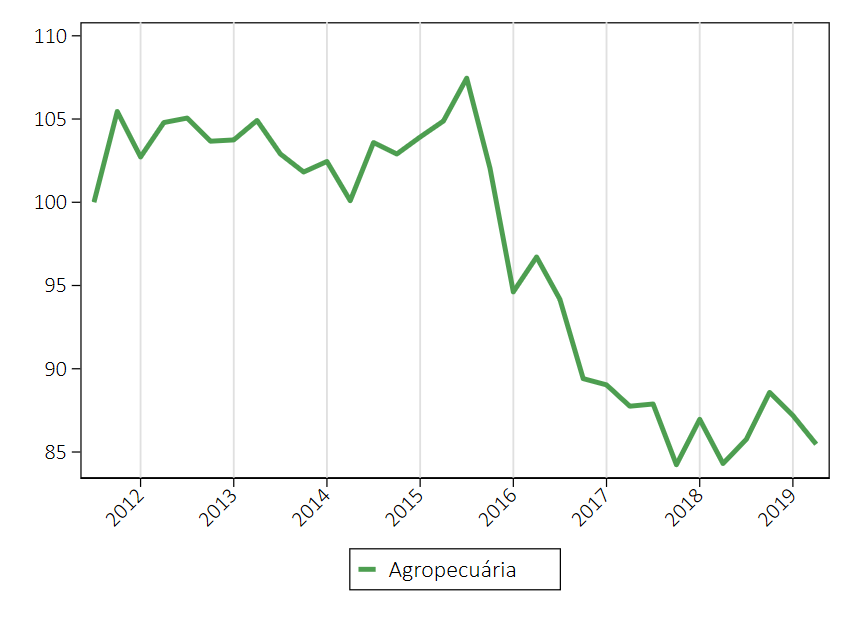
\includegraphics[width=.85\linewidth]{./../analysis/output/_graph_1.png}
  \label{_importancia_relativa}
  \caption{{Crescimento relativo do número de ocupações (1T de 2012 $=$ 100)}}
\end{figure}
\end{frame}

\begin{frame}[label=_graph_2]
\textit{\hyperlink{_graph_2}{\beamerbutton{Voltar}}}
\begin{figure}
  \centering
  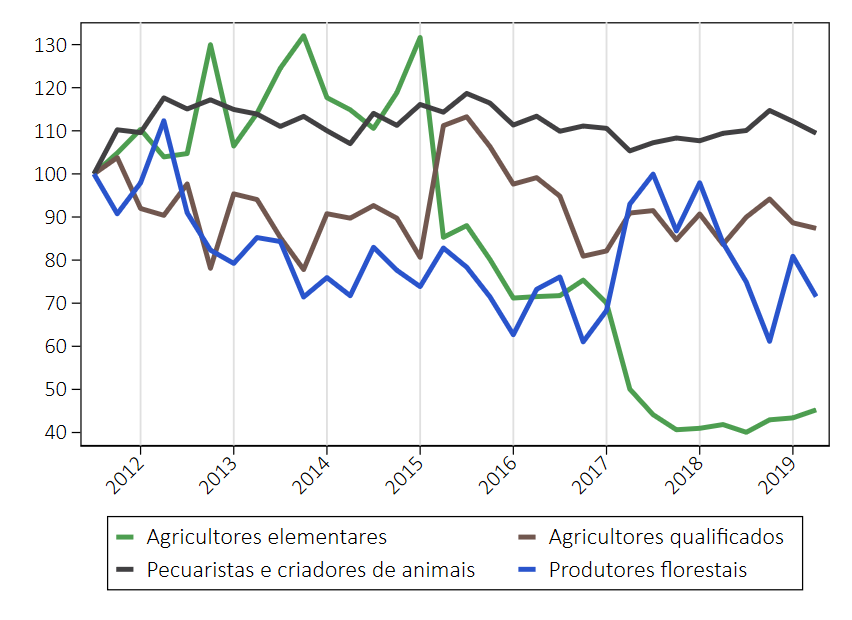
\includegraphics[width=.85\linewidth]{./../analysis/output/_graph_2.png}
  \label{_importancia_relativa}
  \caption{{Crescimento relativo do número de ocupações (1T de 2012 $=$ 100)}}
\end{figure}
\end{frame}


\begin{frame}[label=amzcod2dig]{}

\begin{table}[H]
\centering
\label{amzcod2dig}
\scalebox{0.75}{
\begin{threeparttable}
\caption{Ocupações que mais cresceram entre 2012 e 2019}
\begin{tabular}{l*{8}{r}}
\midrule \midrule
 &  \multicolumn{3}{c}{\textbf{Variação 2012-19}} & \multicolumn{4}{c}{\textbf{2019}} \\
\cmidrule(lr){2-4} \cmidrule(lr){5-8}
 & Emp. & Emp. & Rendi. & { Emp.} & { Rendi. } & {Formal} & {Privado} \\
                    &       total&        (\%)&        (\%)&    {total }&     {(R\$)}&        (\%)&        (\%)\\
\hline
\\
\multicolumn{3}{l}{\textbf{Ocupações que mais cresceram:}}  \\
\\
Vendedores          &     606.932&        62,7&        -5,7&   1.574.725&       1.378&        35,7&        99,9\\
Serviços e cuidados pessoais&     143.490&        23,5&        -6,3&     754.816&       1.056&        32,4&        82,6\\
Profissionais da saúde&     100.787&        40,7&        -2,6&     348.642&       3.327&        72,9&        31,5\\
Escriturários      &      88.196&        23,2&         6,7&     467.694&       1.948&        72,9&        53,8\\
Montadores e condutores de veículos&      69.529&        12,1&        -6,6&     642.256&       1.789&        53,1&        92,1\\
\\
\multicolumn{3}{l}{\textbf{Ocupações em agropecuária:}}  \\
\\
Pecuaristas e criadores de animais&      16.016&         2,0&        18,7&     799.419&       1.118&        22,7&       100,0\\
Produtores florestais&     -38.877&       -28,1&        -3,4&      99.690&         503&        10,6&        99,9\\
Agricultores qualificados&     -44.654&        -6,7&        15,4&     618.948&         604&         9,1&        99,9\\
Agricultores elementares&    -254.690&       -59,0&        55,0&     176.646&         498&         7,7&        99,9\\
\\
\hline
\\
\textbf{Total Amazônia Legal}               &     537.822&         5,3&         3,4&  10.632.195&       1.692&        40,6&        84,2\\
\\
\bottomrule
\end{tabular}
\begin{tablenotes}
\item \scriptsize{Fonte: com base nos dados da PNAD Contínua, IBGE}
\end{tablenotes}
\end{threeparttable}
}
\end{table}

\end{frame}

\begin{frame}[label=amzcod2dig]{}

\begin{table}[H]
\centering
\label{amzcod2dig}
\scalebox{0.56}{
\begin{threeparttable}
\caption{Ocupações que mais cresceram entre 2012 e 2019}
\begin{tabular}{l*{8}{r}}
\midrule \midrule
 &  \multicolumn{3}{c}{\textbf{Variação 2012-19}} & \multicolumn{4}{c}{\textbf{2019}} \\
\cmidrule(lr){2-4} \cmidrule(lr){5-8}
 & Emp. & Emp. & Rendi. & { Emp.} & { Rendi. } & {Formal} & {Privado} \\
                    &       total&        (\%)&        (\%)&    {total }&     {(R\$)}&        (\%)&        (\%)\\
\hline
Vendedores          &     606.932&        62,7&        -5,7&   1.574.725&       1.378&        35,7&        99,9\\
Serviços e cuidados pessoais&     143.490&        23,5&        -6,3&     754.816&       1.056&        32,4&        82,6\\
Profissionais da saúde&     100.787&        40,7&        -2,6&     348.642&       3.327&        72,9&        31,5\\
Escriturários      &      88.196&        23,2&         6,7&     467.694&       1.948&        72,9&        53,8\\
Montadores e condutores de veículos&      69.529&        12,1&        -6,6&     642.256&       1.789&        53,1&        92,1\\
Serviços jurídicos, sociais e culturais&      62.548&        38,5&         1,6&     225.002&       3.947&        43,1&        68,0\\
Profissionais do ensino&      39.679&         8,3&        14,3&     519.988&       3.206&        67,7&        19,6\\
Policiais, bombeiros e forças armadas&      31.821&        45,6&        34,5&     101.582&       5.433&       100,0&         0,0\\
Técnicos de eletricidade e eletrônica&      28.535&        37,2&       -10,2&     105.250&       1.594&        45,7&        96,4\\
Domésticos         &      27.850&         3,4&         9,3&     852.797&         878&        35,3&        87,3\\
Profissionais em alimentação&      22.248&        36,1&       -13,7&      83.949&         905&        37,0&        93,0\\
Artesões e artes gráficas&      18.850&        34,3&        -6,4&      73.854&         879&        22,7&        99,5\\
Administração pública e de empresas&      17.236&        31,0&       -15,9&      72.856&       4.877&        77,5&        77,1\\
Coletores de lixo   &      16.417&        18,7&       -16,1&     104.132&         925&        42,7&        74,3\\
Pecuaristas e criadores de animais&      16.016&         2,0&        18,7&     799.419&       1.118&        22,7&       100,0\\
Atendimento direto ao público&       6.524&         5,0&         2,6&     136.212&       1.342&        61,8&        82,2\\
Serviços de TI e comunicação&       2.854&         5,9&         3,6&      51.622&       2.712&        71,3&        85,6\\
Operários de processamento e instalações&     -13.572&        -2,5&       -14,9&     526.651&         936&        31,8&        99,6\\
Apoio administrativo&     -16.871&       -15,0&         5,9&      95.423&       1.735&        84,8&        86,5\\
Serviços financeiros e administrativos&     -17.161&        -9,4&        17,8&     164.663&       3.659&        59,7&        71,9\\
Profissionais de segurança&     -24.588&       -10,2&        15,9&     216.267&       2.114&        74,3&        53,0\\
Trabalhadores no governo&     -25.315&       -44,2&         4,2&      31.909&       5.859&        43,1&        25,2\\
Produtores florestais&     -38.877&       -28,1&        -3,4&      99.690&         503&        10,6&        99,9\\
Agricultores qualificados&     -44.654&        -6,7&        15,4&     618.948&         604&         9,1&        99,9\\
Cientistas e engenheiros&     -59.432&       -25,8&        16,2&     170.971&       3.625&        65,7&        83,0\\
Operários da construção, metalurgia e indústria&     -65.240&        -4,8&        -4,7&   1.292.188&       1.314&        31,0&        98,5\\
Ambulantes          &     -90.586&       -60,0&        -7,0&      60.333&         950&         6,9&        99,9\\
Dirigentes e gerentes&    -110.705&       -29,6&        -4,1&     263.712&       4.459&        64,9&        88,1\\
Agricultores elementares&    -254.690&       -59,0&        55,0&     176.646&         498&         7,7&        99,9\\
\hline
\textbf{Total}               &     537.822&         5,3&         3,4&  10.632.195&       1.692&        40,6&        84,2\\
\bottomrule
\end{tabular}
\begin{tablenotes}
\item \scriptsize{Fonte: com base nos dados da PNAD Contínua, IBGE}
\end{tablenotes}
\end{threeparttable}
}
\end{table}

\end{frame}


\section{Comentários}

\frame
{
\begin{center}
	\vfill
	\textbf{Obrigado!}
	\\
	\vfill     
\end{center}
}

\end{document}

